\documentclass{article}
\usepackage{../fasy-hw}
\usepackage{algpseudocode}
\usepackage{hyperref}
\usepackage{graphicx}

%% UPDATE these variables:
\renewcommand{\hwnum}{0}
\title{Discrete Structures, Homework \hwnum}
\author{Ben Miller}
\collab{\todo{list your collaborators here}}
\date{due: 30 August 2021}

\graphicspath{ {./} }

\begin{document}

\maketitle

\todo{citations}

This homework assignment should be
submitted as a single PDF file both to D2L and to Gradescope.

General homework expectations:
\begin{itemize}
      \item Homework should be typeset using LaTex.
      \item Answers should be in complete sentences and proofread.
      \item You will not plagiarize, nor will you share your written solutions
            with classmates.
      \item List collaborators at the start of each question using the
            \texttt{collab} command.
      \item Put your answers where the \texttt{todo} command currently is (and
            remove the \texttt{todo}, but not the word \texttt{Answer}).
\end{itemize}

%%%%%%%%%%%%%%%%%%%%%%%%%%%%%%%%%%%%%%%%%%%%%%%%%%%%%%%%%%%%%%%%%%%%%%%%%%%%%%
\collab{N/A}
\nextprob{Getting to Know You}

Answer the following questions:
\begin{enumerate}
      \item What is your elevator pitch?  Describe yourself in 1-2
            sentences.
            
            \paragraph{Answer} My name is Ben Miller and I am in my third year of the bachelor's to master's 
            computer science track at MSU. I am an undergraduate research assistant under Dr. Maher, and I like to
            code with raspberry pi's and work with data.
            
      \item What was your favorite CS class so far, and why?
            
            \paragraph{Answer} My favorite CS class so far was probably Data Mining. It covered a lot of interesting topics,
            was just about the right difficulty level, and gave me a lot of skills that I already have gotten use out of.
            
      \item What was your least favorite CS class so far, and why?
            
            \paragraph{Answer} My least favorite CS class was Discrete Math, which doesn't bode well for this course.
            I still liked the course, but I felt like I only had a passing understanding for half of the topics.
            I'm working hard on getting it all down now, so I'm doing a bit of catching up.
            
      \item Why are you interested in taking this course?
            
            \paragraph{Answer} I thought this course would be interesting and I'm planning on taking 532 next semester.
            Understading algorithms is incredibly useful and however hard some topics may be, I find them quite rewarding.
            
      \item What is your biggest academic or research goal for this semester (can
            be related to this course or not)?
            
            \paragraph{Answer} I want to be comfortable with each topic in each of my courses. For research, I want to 
            use the techniques we've developed to get a spacial clue about our audio data. So far, our alignmnet
            methods have been too inaccurate to draw any spacial conclusions.
            
      \item What do you want to do after you graduate?
            
            \paragraph{Answer} I don't really know. I want to work on something meaningful and pay off my student loans.
            
      \item What was the most challenging aspect of your coursework last semester?
            
            \paragraph{Answer} The most challenging aspect of my coursework last semester was the group work in my writing
            class. Half of the group members did not contribute at all and it was very frustrating.
            
      \item Is your photo in D2L a recognizable photo of yourself?  (Note: the
            answer should be ``Yes'').
            
            \paragraph{Answer} Yes
            
\end{enumerate}


%%%%%%%%%%%%%%%%%%%%%%%%%%%%%%%%%%%%%%%%%%%%%%%%%%%%%%%%%%%%%%%%%%%%%%%%%%%%%%
\collab{N/A}
\nextprob{Discussion Board}

Make a post in the class discussion board. No answer needs to be written here.
But, for bonus points, include a screenshot of your post.

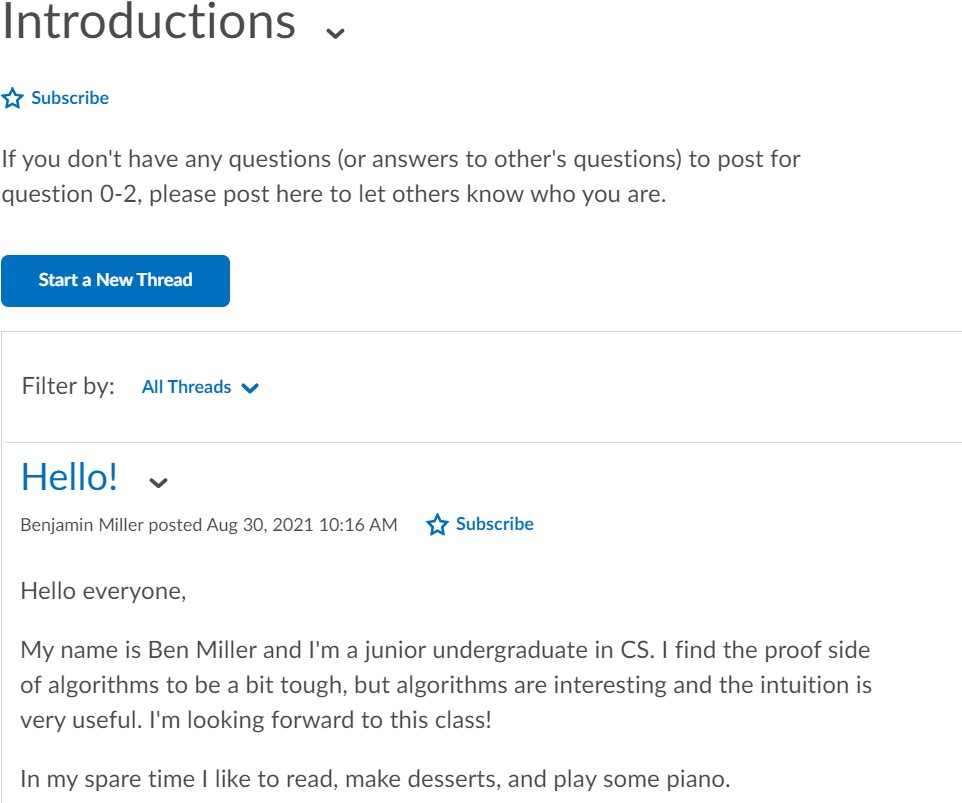
\includegraphics{post_screenshot.jpg}


%%%%%%%%%%%%%%%%%%%%%%%%%%%%%%%%%%%%%%%%%%%%%%%%%%%%%%%%%%%%%%%%%%%%%%%%%%%%%%
\collab{}
\nextprob{Plagiarism}

\begin{enumerate}

      \item In this class, please properly cite all resources that you use. Please
            write your own definition of plagiarism here.  Remember to cite all
            sources!
            
            \paragraph{Answer}
            Plagiarism is using the ideas or work of another as one's own without giving them credit.  
            \footnote{I used google's definition as a reference, which in turn is from Oxford Languages.}
            
      \item If you have observed plagiarism or cheating in a classroom (either as
            an instructor or as a student), explain the situation and how it made
            you feel.  If you have not experienced plagiarism or cheating or if you
            would prefer not to reflect on a personal experience, find a news
            article about plagiarism or cheating and explain how you would feel if
            you were one of the people involved.
            
            \paragraph{Answer}
            In high school, there was a girl two grades above me that was caught plagiarizing
            another student's work twice. Both times it was a larger paper in an English class.
            The first time, she was made to redo the paper and there were no other repurcussions.
            The sedond time, she was disciplined the same way. She may have been dropped a letter grade
            the second time, but either way, it wasn't that bad. 
            
            Most of thought that if it was somebody else that plagiarized twice, they would have gotten expelled
            because that is what it said in the handbook. We all knew that she plagiarized many other assignments
            but never got caught. As a student, I understand not wanting to do an assignment and it doesn't really
            affect me directly, but I still felt like it devalued the class a little. For more professional settings,
            the plagiarism would be a bigger deal. In that setting, it was more a case of "you're only cheating yourself."
            
            
\end{enumerate}

%%%%%%%%%%%%%%%%%%%%%%%%%%%%%%%%%%%%%%%%%%%%%%%%%%%%%%%%%%%%%%%%%%%%%%%%%%%%%%
\collab{}
\nextprob{Edges in Trees}

Prove or disprove the following statement: Every tree with one or more
nodes/vertices has exactly $n-1$ edges, where $n$ is the number of vertices in
the tree.

\paragraph{Answer}
\footnote{With help from https://www.geeksforgeeks.org/some-theorems-on-trees/}

A tree is a graph with no circuits, so only one edge is added for each node added

let $m$ be the number of edges.

For every integer $n \geq 1, n - 1 = m$

{\bf Basis:} n = 1 is true as $1 - 1 = 0$. n = 2 is true as $2-1=0$

{\bf Inductive Assumption:} Assume that $n - 1 = m$ is true.

      {\bf Inductive Step:} $$(n+1) -1 = m $$
$$(n+1) -1 = (n +1) - 1$$
$$n=n$$
$$n=m +1$$
$$n-1=m$$



%%%%%%%%%%%%%%%%%%%%%%%%%%%%%%%%%%%%%%%%%%%%%%%%%%%%%%%%%%%%%%%%%%%%%%%%%%%%%%
\collab{}
\nextprob{Big-O}

Use the definition of big-O notation to prove that $f(x)=n^2 + 3n -2$ is
$O(n^2)$.

\paragraph{Answer}
\footnote{Used past work from Discrete Mathematics to help}

For $n \ge 1$, $ n^2 + 3n -2 \leq A n^2$

Hence $f(x) \leq A \cdot n^2$, when $A = 1$ and $n \geq a = 1$

Therefore, $f(x)=n^2 + 3n -2$ is $O(n^2)$.

\paragraph{}

%%%%%%%%%%%%%%%%%%%%%%%%%%%%%%%%%%%%%%%%%%%%%%%%%%%%%%%%%%%%%%%%%%%%%%%%%%%%%%
\collab{}
\nextprob{If/Then Statements}
Consider the following statement: If $a$ and $b$ are both even numbers, then $ab$ is
an even number.
\begin{enumerate}
      \item What is the definition of an odd number?
            
            \paragraph{Answer} If a number x is odd, then x will not be an integer if divided by 2.
            \footnote{Used past work from Discrete Mathematics to help}
            
      \item What is the definition of an even number?
            
            \paragraph{Answer} If a number x is even, then x will be an integer if divided by 2.
            
      \item What is the contrapositive of this statement?
            
            \paragraph{Answer} If $ab$ is not an even number, then $a$ or $b$ are not an even number.
            
      \item What is the converse of this statement?
            
            \paragraph{Answer} If $ab$ is an even number, then $a$ and $b$ are both even numbers.
            
      \item Prove this statement.
            
            \paragraph{Answer} Because $a$ is even, let $ a= 2c$ where $c$ is an integer.
            Because $b$ is even, let $ b= 2d$ where $d$ is an integer.
            
            $ab = (2c) \cdot (2d)$
            
            $ab = 4cd$
            
            $\frac{4cd}{2} = 2cd$
            
            Therefore $ab$ is an even number
            
            
            \paragraph{}
            
\end{enumerate}



%%%%%%%%%%%%%%%%%%%%%%%%%%%%%%%%%%%%%%%%%%%%%%%%%%%%%%%%%%%%%%%%%%%%%%%%%%%%%%
\collab{}
\nextprob{Sorting}
Consider your favorite sorting algorithm.

Bubblesort
\begin{enumerate}
      \item \emph{What} is the problem that this algorithm solves?
            
            \paragraph{Answer} Bubblesort is the most fun to watch. I find it very
            satisfying to watch the items bubble to the top.
            Bubble sort is very fast at bringing low items to the top, but it is quite
            slow at bringing high items to the bottom. There is a variant called Cocktail sort
            that bubbles both directions, but it isn't as fun. Bubble sort also very quickly checks
            to see if the array is already sorted during the first step.
            
      \item \emph{How} does it work? (Hint: give pseudocode!)
            
            \paragraph{Answer}
            \footnote{With help from \href{https://en.wikipedia.org/wiki/Bubble_sort}{wikipedia}}
            
            \begin{algorithm}\caption{\textsc{Bubblesort}($array$)}\label{alg:seb}
                  {\bf Input:} array $array$ of sortable items\\
                  {\bf Output:} Sorted array
                  \begin{algorithmic}[1]
                        \State $A \gets length(array)$
                        \State $P \gets 0$
                        \State $SwapOcurred \gets true$
                        \While{$SwapOcurred == true$}
                        \State $SwapOcurred \gets false$
                        \For{$i$ in $1$ to $n-1 - P$}
                        \If {$array[i-1] > array[i]$}
                        \State $swap(array[i-1], array[i])$
                        \State $SwapOcurred \gets true$
                        \EndIf
                        \EndFor
                        \State $ P \gets P + 1$
                        \EndWhile\\ 
                        \Return $array$
                  \end{algorithmic}
            \end{algorithm}
            
      \item \emph{How fast} does it work?  Give the asymptotic running time.
            Note: typically, you will give this as the worst-case running time.
            However, if you chose quicksort or another randomized algorithm, please
            give both the worst-case running time and the expected running time.  No
            justification of the running time is needed.
            
            \paragraph{Answer} The running time is $O(n^2)$
            
      \item \emph{Why} does this work? Typically, this will be given as a loop
            invariant proof.  For this HW, explain why it works informally, in your
            own words.
            
            \paragraph{Answer}
            Bubble sort always starts at the first item, compares it to the next item,
            and swaps them if the first item is greater. Then, it shifts up once and repeats
            the process. 
            
            let $a$ be the length of the array and let $b$ be the number of passes.
            
            In this manner, the largest element in the array up to position $[a-b]$ is always brought
            to position $[a - b]$. By checking to see if a swap occured on each pass, we can check 
            if the array is sorted before actually performing each pass.
            
\end{enumerate}


Note: in all future HWs, if you are asked to come up with an algorithm, you are
expected to give an algorithm that beats the brute force (and, if possible, of
optimal time complexity). With your algorithm, please provide the following:
\begin{itemize}
      \item \emph{What}: A prose explanation of the problem and the algorithm,
            including a description of the input/output.
      \item \emph{How}: Psuedocode, referenced from within the prose explanation.
      \item \emph{How Fast}: Runtime, along with justification.  (Or, in the
            extreme, a proof of termination).
      \item \emph{Why}: Statement of the loop invariant for each loop.
\end{itemize}

\end{document}
